\chapter{Assembly and Dynamics of Rod-Shaped Colloids}
\section{Introduction}

When one is first presented with the different dimensions of anisotropy proposed by 
Glotzer and Solomon (Figure~\ref{fig:glotzer-dimensions},\ref{glotzer-solomon-assembly}), the
potential variety of particle types can be overwhelming. It is therefore useful to begin by studying 
particles which draw from only one or two of these anisotropy dimensions. To this end, our
initial study has focused on particles which vary only in the dimension of 
aspect ratio, i.e. colloidal rods. This study covers the fabrication of both single-component and 
Janus rods by stop-flow lithography, the study of rod diffusion by particle tracking, and the basics
of self-assembly for Janus rods in different solvents.

%\tempfigure{Colloidal rod examples}
%\begin{itemize}
%\statement{Natural rod systems}
%\statement{Systems studied by Solomon}
%\statement{Janus colloids: Granick}
%\statement{Interest in Janus rods}
%\end{itemize}

\section{Experimental Procedure}

Colloidal rods were fabricated by stop-flow lithography (SFL) as described in section~\ref{sec:SFL} using
hydrophobic and hydrophilic monomer solutions.  

\subsection{Microchannel device fabrication}

Particle fabrication was carried out in Y-junction microchannel devices (Figure~\ref{fig:device-desig}).
The primary channel of these devices had a typical 
height of 7 \microns, width of 200 \microns, and length of 3000-5000 \microns. These dimensions were selected
to faciliate the fabrication of large numbers of particles with small size in all dimensions: the low height
facilitated small-particle fabrication by limiting the height of the particles, while the comparatively large
width allowed many particles to be fabricated simultaneously. Multiple entrances were defined to allow up to three
monomer streams to be simultaneously flowed, with a single exit point for collecting particles.

\subsubsection{Photoresist masters}
Positive-relief photoresist master templates were fabricated by UV photolithography. A thin film
of SU-8 2007 photoresist (Microchem) was laid down on a clean Si wafer via spin-coating at 3000 rpm to produce a 
7 \microns layer. Next, a ``soft bake'' was carried out by heating the wafer on a hot plate at 120\degC
for five minutes to evaporate the photoresist solvent.  The device features were patterned by exposing the 
photoresist to UV light ??? for 40 s through a photomask defining the device design. A ``hard bake'' step
was then carried out by heating the wafer at 120\degC for ten minutes, to cure the photoresist in the exposed areas.
Finally, the wafer was immersed in SU-8 developer (Microchem) and agitated for two minutes to remove the unexposed
photoresist, then rinsed with isopropyl alcohol (IPA).

After fabrication, photoresist masters were subjected to a fluorinated silane vapor coating to inhibit adhesion
between the SU-8 template and the elastomer to be cast. Masters were placed in a small dessicator (Fisher Scientific)
along with an open container of (tridecafluoro-1,1,2,2-tetrahydrooctyl) trichlorosilane (Gelest, Inc.)
This dessicator's vacuum port was then connected to a single-stage vacuum pump and evacuated for two hours to produce
a silane coating.

\subsubsection{Elastomer device construction}

Microchannel devices were constructed from polydimethylsiloxane (PDMS, Dow Corning, Sylgard 184). PDMS
elastomer and curing agent were mixed at a ratio of 10:1 by weight, and pored over the photoresist master 
in a plastic petri dish to a depth of about 2 mm.  PDMS was also spun-coat onto a 48 x 60 mm \#1 coverslip (Gold Seal)
to form the substrate for the device.
Both of these  were then baked at 65\degC for six hours or more to cure
the PDMS.  

Once the PDMS was fully cured, a razor blade was used to carefully cut out a section which encompassed some or all of
the microchannels defined on the photoresist master. This section was then peeled up from the master, revealing
a block of PDMS which contained negative features defining the top and sides of the microchannels.
For each microchannel, three small holes (\~ 0.5 mm) were punched at each entrance using a syringe press, and a larger
hole (\~ 3 mm) was punched at the exit using a biopsy punch.

For each of the ``top side'' PDMS block and the PDMS-coated glass substrate, the PDMS surface was rinsed with 
deionized water and IPA.  Following this, small particles were removed by first laying down and then peeling up
Scotch Magic brand transparent tape.~\ref{rogers-tape-ref}  Each section was then placed below a UV light-emitting
diode with the channel surface facing the diode, and exposed to UV light for ten minutes to promote PDMS-PDMS
adhesion.  After UV exposure, these sections are then firmly pressed together with the channel surface of the top
block against the PDMS-coated surface of the substrate.  The resulting device is then baked at 100\degC for one hour
to promote device bonding.

\subsection{Materials}
The hydrophobic solution was composed of 95 v/o 
tri(methylol propane) triacrylate (TMPTA, Sartomer) and 5 v/o Darocur 1173 photoinitiator (Ciba), 
with 0.005 wt\% methacryloxyethyl thiocarbamoyl rhodamine B (Polysciences) as a cross-linking 
fluorescent dye.
The hydrophilic solution was composed of either 20 mol ethoxylated tri(methylol propane) triacrylate (20-ETMPTA,
Sartomer) or poly(ethylene glycol) diacrylate (PEGDA, $M_n$ = 700, Sigma Aldrich) at 80 v/o, 
15 v/o deionized water, and 5 v/o Darocur 1173 photoinitiator, with 0.005 wt\% 
3,8-dimethacryloyl ethidium bromide (Polysciences) as a cross-linking fluorescent dye.


\subsection{Mask design}
Masks used for single-component fabrication contained two-dimensional arrays of identical aligned 
rods, with a separation in each direction equal to twice the length of the rod to avoid inter-particle
curing (Figure~\ref{fig:rod-masks}(a)). These arrays were designed to maximize the number of 
rods cured per cycle by making them large enough to, at minimum,
cover the field stop aperture for the transmission of the UV beam. This circular aperture 
had a diameter of 1.5 inches.  For example, the photomask containing 500~\microns rod features
was a twenty-by-twenty array, with the 1 mm separation ensuring that the mask area was large enough to
use the full available beam.  
Masks used for Janus fabrication contained only a single line of rod features, with the rods parallel to one 
another and aligned perpendicular to the axis of the line (Figure~\ref{fig:rod-masks}(b)).  Spacing on these 
masks was the same as for single-component fabrication.


\subsection{SFL experiment}
UV exposure and experimental imaging for small-rod fabrication was carried out using a 60x 
oil-immersion objective lens (Olympus America), with an additional 1.6x lens added to the beam path for
the fabrication of smaller rods.  Using the 60x objective, a demagnification factor of approximately 
33 was typically observed between the mask and the resulting rods; i.e., a rod of 500~\microns length defined on
the photomask would typically result in the fabrication of a 12~\microns rod in the microchannel.

Microchannel flow was driven by gas pressure supplied by a house nitrogen line or a compressed air tank 
(SJ Smith Welding Supply). Pressure control was achieved using a custom-built pressure box, consisting of
four computer-controlled regulators and four duplex valves connected to a USB
controller (National Instruments) allowing for 
up to four independent pressures driving up to eight separate lines. UV light was supplied by a ?? W mercury lamp
connected in fluorescence microscope configuration, with exposure time controlled using a Lambda SC 
electronic shutter (Sutter Instruments).

The SFL experiment was driven using LabView software (National Instruments) with a custom
interface (Figure~\ref{fig:sfl-labview}). The process
flow of an SFL experiment is illustrated in Figure~\ref{fig:sfl-flowchart}, and consists of the following steps:

\begin{enumerate}
\item Specify ``flow time'' $t_{flow}$, ``pause time'' $t_{pause}$, and exposure time $t_{expose}$.
\item Set pressure for each port on electronic regulators.
\item Until the experiment is stopped:
\begin{enumerate}
\item Open valves. Wait $t_{flow}$.
\item Close valves. Wait $t_{pause}$.
\item Open shutter. Wait $t_{expose}$.
\item Close shutter. Repeat.
\end{enumerate}
\end{enumerate}

For a schematic of the SFL experimental setup, see Figure~\ref{fig:sfl-schematic}.
For each monomer solution, a 10-100\uL pipette tip (Eppendorf) was filled with approximately 60\uL of solution.
A silicone tube was connected at one end to the output of one valve of the pressure box, and the other end
was inserted into the top of the pipette tip.  The bottom of the pipette tip was then inserted into one of the
small entrance holes in the microchannel device.  This device was the placed on above the microscope objective,
and the microscope was focused such that the focal place was inside the channel.  After starting the 
experiment, the shutter was allowed to open and the fine focus was adjusted manually to optimize
curing conditions. Optimization was judged by visual inspection of the resulting particles. 

Single-component rods were fabricted using the central entrance channel to supply monomer to the system, 
leaving the other two entrances unused. Typical experimental settings for these experiments were pressure
8 psi, flow time 1.5 s, and pause time 2 s.  Exposure times for PEGDA or 20-ETMPTA were typically 0.05-0.15 s
depending on the mask dimensions, while exposure times for TMPTA were typically 0.2-0.3 s to account for
the less favorable curing behavior of the hydrophobic monomer.  The fabrication of smaller rods generally
necessitated slightly higher exposure times.  

Janus rods were fabricated using the two side entrance channels to supply each type of monomer solution,
with the central channel left unused.  (All three channels were used for fabricating branched Janus particles; see
section~\ref{sec:SFLx3}.)  Typical experimental settings for these experiments were pressure 7 psi on each side, 
flow time 2 s, pause time 2 s, and exposure time 0.2-0.3 s depending on the mask dimensions.
The two monomer streams would enter the main channel on either side, and form
an interface along the center of the channel (Figure~\ref{fig:Janus-channel}). Because the hydrophobic and
hydrophilic streams were immiscible and the microchannel flow took place in the laminar flow regime~\ref{?}, 
this interface persisted for several hundred microns down the channel.
During fabrication, the curing regions would be aligned such that each rod straddled this interface,
producing rods which incorporated both materials.

In either case, the resulting particles were ejected at the end of the experiment into the final reservoir, which
was left empty to allow collection of the maximum volume of particles possible.


\tempfigure{Photo of SFL setup; SFL flowchart; example experiment}
\begin{itemize}
\done{Microscope setup}
\done{Pressure system--Rob}
\done{LabView controller for SFL}
\done{Design of microfluidic devices for up to 3-stream SFL}
\done{Fabrication of microfluidic devices}
\end{itemize}


\subsection{Particle Collection}


\subsection{Diffusion Measurements}
\begin{itemize}
\done{Confocal microscopy setup}
\done{Space and time resolution requirements}
\done{Fluorescence requirements}
\end{itemize}

\section{Results and Discussion}

\tempfigure{Resolution test mask; image of resulting particles}
\subsection{Resolution}
\begin{itemize}
\done{Limiting factors for SFL resolution: mask design, optics, flow effects}
\notdone{Resolution limits constrained by 60X lens--need to redo this (~1 hour work)}
\done{Resolution limits for Janus rods--interface effects}
\end{itemize}

\tempfigure{Image of rod tracking}
\tempfigure{Plots of translational and rotational diffusion data}
\subsection{Translational and Rotational Diffusion}
\begin{itemize}
\done{Particle collection--PEGDA vs TMPTA}
\done{Compare particle/solvent/surface effects}
\notdone{2D diffusion size series: TMPTA in toluene (additional experiments may be required)}
\notdone{Analyze diffusion data for rods (partially done).}
\end{itemize}

\tempfigure{Show fabricated Janus rods of various sizes.}
\tempfigure{Assembly of rods in various solvents}

\begin{figure}
\begin{center}
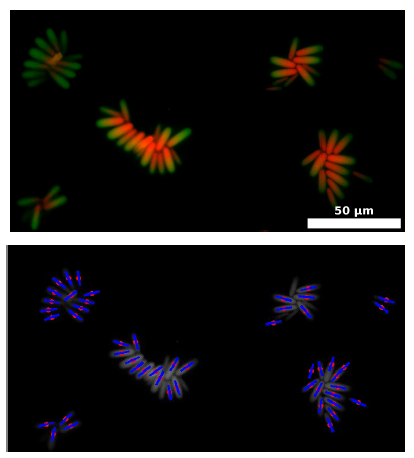
\includegraphics{figures/assembled-janus-tracked.png}
\end{center}
\caption{(a) Janus rods which have self-assembled into ordered 
clusters are identified and separated, and (b) their 
positions and orientations are labeled.}
\label{fig:assembled-janus-tracking}
\end{figure}

\subsection{Self-Assembly of Janus Rods}
\begin{itemize}
\done{Fabrication of Janus rods: various sizes (figure)}
\done{Comparison of self-assembly in various solvents (figure)}
\done{Small clusters vs large structures}
\done{Alignment of assembled rods}
\done{Image segmentation for analyzing structures}
\notdone{Some more good-looking images may be required}
\end{itemize}
